\documentclass[compress]{beamer}
\usepackage{ifthen}
\usepackage{verbatim}
\usepackage{array}

\xdefinecolor{lightyellow}{rgb}{1.,1.,0.25}
\xdefinecolor{darkblue}{rgb}{0.1,0.1,0.7}

\setbeamertemplate{navigation symbols}{}
\setbeamertemplate{headline}{\mbox{ } \hfill
\begin{minipage}{5.5 cm}
\vspace{-0.75 cm} \small
\end{minipage} \hfill
\begin{minipage}{4.5 cm}
\vspace{-0.75 cm} \small
\begin{flushright}
\ifthenelse{\equal{\insertpagenumber}{1}}{}{Jim Pivarski \hspace{0.2 cm} \insertpagenumber/\pageref{numpages}}
\end{flushright}
\end{minipage}\mbox{\hspace{0.2 cm}} \hspace{0.01 cm} \vspace{-1.05 cm}}

\newcommand{\s}[1]{{\mbox{\scriptsize #1}}}

\begin{document}
\begin{frame}
\vfill
\begin{center}
\textcolor{darkblue}{\Large Barnstorming/Strawman ROOT 7 Graphics}

\vfill
\begin{columns}
\column{0.3\linewidth}
\begin{center}
\large
Jim Pivarski
\end{center}
\end{columns}

%% \begin{columns}
%% \column{0.3\linewidth}
%% \begin{center}
%% \scriptsize
%% {\it Fermilab}
%% \end{center}
%% \end{columns}

\vfill
January 28, 2016

\end{center}
\end{frame}

\small

\begin{frame}
\frametitle{Where I'm coming from}
I'm starting my work for DIANA-HEP, in the exploratory phase of designing a project.

\vfill
DIANA-HEP goals (subset relevant to this talk):
\begin{itemize}
\item Bring industry-standard software and techniques into HEP
\begin{itemize}
\item to relieve maintenance effort within HEP by using software that is maintained by a large, open-source community,
\item for better interoperability with industry-standard tools (particularly ``Big Data'' frameworks and machine learning),
\item to prepare HEP students for a broader range of career options.
\end{itemize}
\item Improve data analysts' user experience and efficiency.
\end{itemize}
\end{frame}

\begin{frame}
\frametitle{Where I'm coming from}

My history:
\begin{description}
\item[1999--2011] HEP student and postdoc, CLEO and CMS
\item[2011--2015] Data scientist and software engineer, Open Data Group
\begin{itemize}
\item Helped clients use Big Data frameworks and machine learning techniques.
\item Developed a standardized interface (\textcolor{blue}{\url{dmg.org/pfa/}}) between the statistical software data scientists use and the production systems that scale them up.
\end{itemize}
\item[now] Project DIANA-HEP
\end{description}

\vfill
\uncover<2>{My interests and goals:
\begin{itemize}
\item Streamline plotting tools and encourage unrestrained plotting.
\item Connect a uniform plotting interface to a variety of Big Data tools, so that a physicist can use them as freely as ROOT.
\end{itemize}}
\end{frame}

\begin{frame}
\frametitle{Where I'm coming from}

Plotting packages I've written (after trying ROOT and many others):

\vspace{0.3 cm}
\renewcommand{\arraystretch}{1.5}
\begin{tabular}{p{0.12\linewidth} p{0.15\linewidth} p{0.65\linewidth}}
\textcolor{blue}{\href{http://github.com/jpivarski/plothon}{Plothon}} & \centering 2006--2008 & Experiments with a Pythonic interface, Qt, GTK+, and later headless graphics: output text for FIG viewers, and in the end, SVG. \\
\textcolor{blue}{\href{http://github.com/jpivarski/svgfig}{SVGFig}} & \centering 2008 & Production-quality package (I used it for physics; thousands of downloads), low-level ``SVG'' and high-level ``Fig'', arbitrary coordinate systems. \\
\textcolor{blue}{\href{http://github.com/opendatagroup/cassius}{Cassius}} & \centering 2011 & Owned by Open Data Group (I used it for my ODG work), introduced categorical and missing data handling for non-physics analyses. \\
\textcolor{blue}{\href{http://github.com/opendatagroup/augustus}{Augustus}} & \centering 2013 & Owned by Open Data Group, extended PMML processing with diagnostic plotting. \\
\end{tabular}
\end{frame}

\begin{frame}
\frametitle{SVGFig examples}

\vspace{-0.4 cm}
\begin{columns}
\column{0.28\linewidth}
\begin{center}

\includegraphics[width=\linewidth]{svgfig_logo.png}

Logo made from non-linear transformations of SVG primitives
\end{center}

\column{0.28\linewidth}
\begin{center}
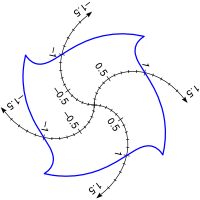
\includegraphics[width=\linewidth]{introduction-10.png}

{\it Any} coordinate system
\end{center}

\column{0.28\linewidth}
\begin{center}
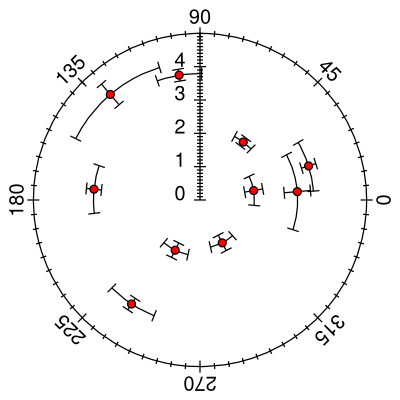
\includegraphics[width=\linewidth]{ExampleRadialPlot.png}

Radial plot from transformation
\end{center}
\end{columns}

\begin{columns}
\column{0.28\linewidth}
\begin{center}
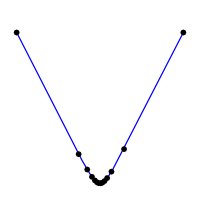
\includegraphics[width=\linewidth]{introduction-8.png}

Curves from adaptive sampling
\end{center}

\column{0.28\linewidth}
\begin{center}
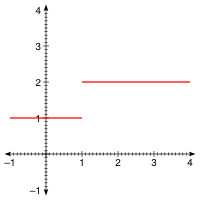
\includegraphics[width=\linewidth]{introduction-9.png}

Discontinuity detection
\end{center}

\column{0.28\linewidth}
\begin{center}
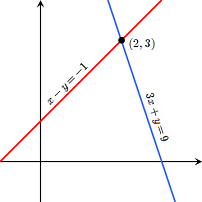
\includegraphics[width=\linewidth]{IntersectingLines.png}

Overlay structure from syntax
\end{center}
\end{columns}
\end{frame}

\begin{frame}
\frametitle{Grammar of Graphics}

\begin{columns}
\column{0.4\linewidth}
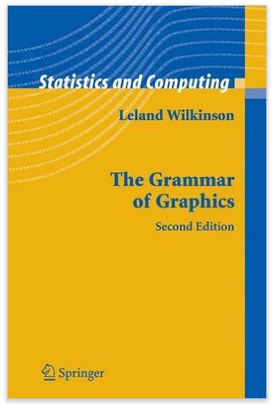
\includegraphics[width=\linewidth]{grammar-of-graphics.png}

\column{0.65\linewidth}
\textcolor{darkblue}{Popular idea:} instead of a function for every type of plot, provide a composable grammar:

\begin{itemize}
\item overlay basic elements;
\item transform coordinates for new plot types;
\item higher level of abstraction that graphics primitives (lines and boxes).
\end{itemize}

\uncover<2>{\textcolor{darkblue}{Examples:}
\begin{itemize}
\item SVGFig (``Fig'' layer)
\item ggplot2 for R
\item supposedly d3 (but it's not high-level)
\end{itemize}}

\end{columns}
\end{frame}

\begin{frame}
\frametitle{Proposal:}

\vspace{0.2 cm}
\textcolor{darkblue}{Add a SVGFig-like plotting interface to ROOT 7.}

\begin{itemize}
\item Headless: ROOT would generate text, not graphics.
\uncover<2->{\begin{itemize}
\item For instance, ROOT acts as a web server supplying responses to REST queries; the ``graphics window'' is a web browser.
\item Could have {\it no dependence} on X11/Cocoa/etc.
\item Faster than X11 forwarding (less data transmitted).
\end{itemize}}

\item Abstract: higher-level than points and lines.
\uncover<3->{\begin{itemize}
\item JSON of plot structure and data: this is the grammar.
\item Include only the data that is to be shown (e.g. bin contents), not how it was made (huge ntuples).
\item Enough information to allow interaction in a browser.
\end{itemize}}

\item Portable: grammar can be standardized and used beyond ROOT.
\uncover<4->{\begin{itemize}
\item Emit same grammar from CMSSW, Hadoop/Spark, a long running Python job, etc.\ to get continuous updates on the content of a data-pull.
\item Emit same grammar from a debugging tool to get {\it statistical distributions} of watched variables.
\item \ldots
\end{itemize}}
\end{itemize}
\end{frame}

\begin{frame}
\frametitle{User experience}
\begin{enumerate}
\item User starts ROOT on local or remote computer.
\item User opens web browser to {\tt localhost:8888} (or something).
\item User's plots appear in web browser do flicker-free refreshing.
\item User saves a plot by invoking Javascript that generates PNG or PDF, or they open the SVG in Inkscape for graphical editing.
\end{enumerate}

\vfill
\hspace{-0.83 cm} \textcolor{darkblue}{\Large Behind the scenes}

\begin{enumerate}
\item ROOT serves an HTML page for each {\tt TCanvas} and a {\tt draw.js} with up-to-date drawing routines.
\item HTML page looks for updates either by polling with tiny AJAX pings or by opening a streaming connection via {\tt readyState 3}.
\item Update is a JSON document describing the plot structure and data.
\end{enumerate}

\vfill
{\bf Issue:} what about services like cmslpc, where users don't know which host they're on and different users can compete for ports?
\end{frame}

\begin{frame}[fragile]
\frametitle{Example grammar}

\begin{columns}
\column{0.56\linewidth}
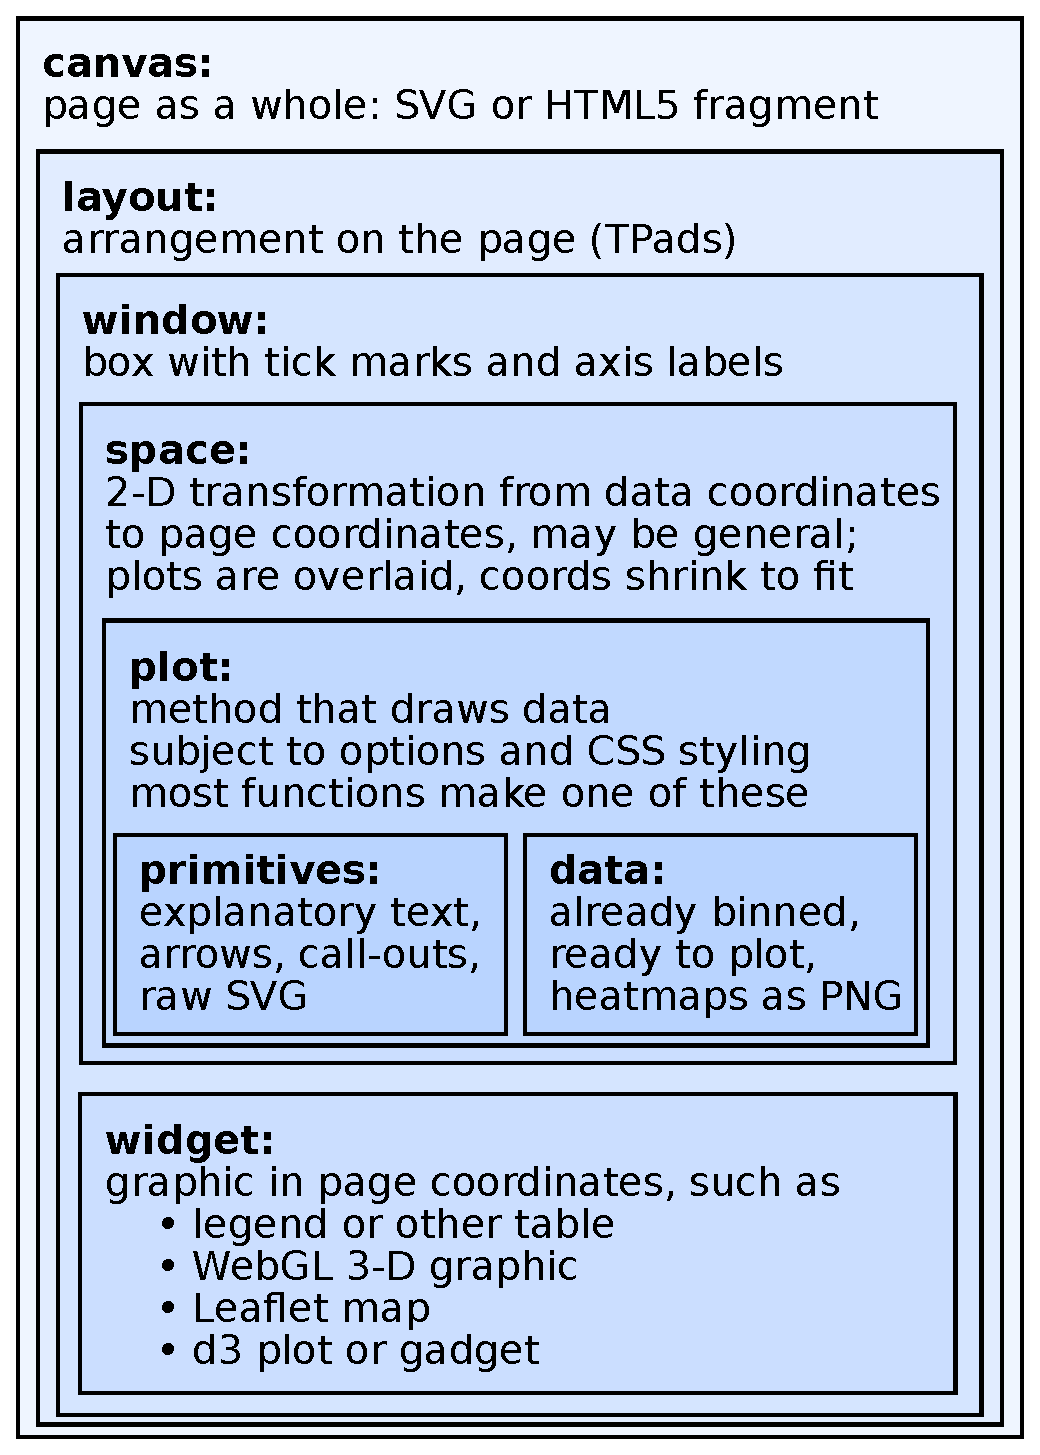
\includegraphics[width=\linewidth]{layers.pdf}

\column{0.5\linewidth}
{\bf Example:}

\vspace{-0.3 cm}
\scriptsize
\begin{verbatim}
{"window": "enclosed",
 "xlabel": "di\\mu mass (GeV/c$^2$)",
 "ylabel": "events per GeV/c$^2$",
 "contents": [
     {"space": "linear-log",
      "xlow": 0,
      "xhigh": 100,
      "ylow": 0.1,
      "yhigh": 120,
      "contents": [
          {"plot": "histogram",
           "numBins": 100,
           "low": 0,
           "high": 100,
           "data": [5, 15, ..., 2],
           "stroke-style":
               "solid 2px black",
           "fill-style":
               "yellow"}
      ]}
 ]}
\end{verbatim}

\vspace{-0.3 cm}
\scriptsize (Missing layers are filled in with defaults.)
\end{columns}
\end{frame}

\begin{frame}
\frametitle{Auxiliary benefits of Javascript}

Although the main target is static PDF for publication, Javascript-enabled SVG or HTML5 has other benefits.

\begin{itemize}
\item Interactivity as an aid to EDM (e.g. pinch to zoom) or for inclusion in end-user interactive dashboards.
\item Can enrich capabilities using community tools:
\begin{itemize}
  \item MathJax (AMS project) renders real LaTeX beautifully,
  \item any gadget from d3's example gallery,
  \item WebGL for smooth, scrollable 3-D objects,
  \item Leaflet, OpenLayers, or other scrollable map,
  \item PDFKit for in-browser SVG $\to$ PDF output,
  \item canvg for SVG $\to$ HTML5 Canvas $\to$ PNG output,
  \item Javascript can be applied to any element, including SVG control points (see Higgs example).
\end{itemize}
\item Javascript can be embedded within C++ (Chromium/V8), Python (PyV8), Java (Rhino/Nashorn), NodeJS, MongoDB, etc.
\item Highly maintained with an emphasis on exact reproducibility.
\end{itemize}
\end{frame}

\begin{frame}
\frametitle{Standardization (last slide)}

In this proposal, the JSON-based grammar is only passed from ROOT to a web browser, along with Javascript code that can interpret it and draw or redraw plots.

\vspace{0.4 cm}
\uncover<2->{But if it's designed well, it could be used in projects beyond ROOT, such as Hadoop/Spark workflows, standalone machine learning packages, etc.\ (anything that lives outside a framework like ROOT or R). This is where DIANA-HEP fits in: I'd be using this as a bridge to Big Data tools.}

\vspace{0.4 cm}
\uncover<3->{Most Big Data tools have {\it no} ability to make plots; many analyses in industry are ``flying blind.'' This could be a part of ROOT that is modular enough to be used outside of ROOT with far-reaching benefits.}

\vspace{0.4 cm}
\uncover<4->{I have experience creating a standard that has been adopted by a standardization committee: Portable Format for Analytics (PFA) is a JSON-encapsulation of scoring engines that is now being maintained by the Data Mining Group.}
\end{frame}

\begin{frame}
\frametitle{Appendix: about SVG}

\vspace{-0.1 cm}
\begin{itemize}
\item Vector-based graphics encoded as XML text, standardized by W3C.
\item Version 1.1 (2003) is now widely supported and robust.

Version 1.2 (2005) was only partially supported.

Version 2 is in working draft, will be ready in December 2016.

\item If the SVG viewer supports Javascript (e.g.\ a web browser), then every element and control point is scriptable. SVG has a specialized DOM for faster (more fully JIT-compilable) scripts.

\item Inkscape is a free, fully featured vector graphics editor whose native format is SVG. I frequantly alternate between manually drawing and programmatically modifying the same graphic as SVG.

\item Limitations:
\begin{itemize}
\item Strictly affine-linear transformations, which affect line thicknesses as well as control points.
\item No universal support for reflowable text yet.
\item No way to determine the size of a text element to avoid overlaps. (Use MathJax to turn all text into paths?)
\item Implementations render zoomed-in pixelmaps differently: some how fatbits while others attempt to smooth.
\end{itemize}

\end{itemize}
\end{frame}

\begin{frame}
\frametitle{Appendix: high-level primitives}
\begin{itemize}
\item Higher-level than raw SVG, for making annotation overlays.
\begin{itemize}
\item For example, an arrow with text with one end in the data-coordinates (to point at a peak) and the other in page coordinates (to keep text from falling out of view).
\end{itemize}
\item Customized sensitivity to the grammar's coordinate systems:

\begin{columns}
\column{0.25\linewidth}
\begin{center}
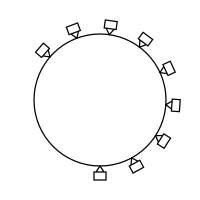
\includegraphics[width=\linewidth]{Version2Announcement_ferris2.png}

fully transformed
\end{center}

\column{0.25\linewidth}
\begin{center}
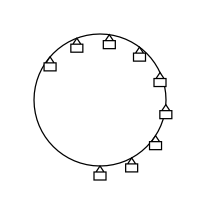
\includegraphics[width=\linewidth]{Version2Announcement_ferris3.png}

position only
\end{center}

\column{0.25\linewidth}
\begin{center}

\includegraphics[width=\linewidth]{Version2Announcement_ferris1.png}

fixed position
\end{center}

\column{0.25\linewidth}
\begin{center}
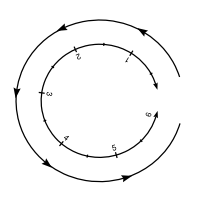
\includegraphics[width=\linewidth]{Version2Announcement_arrowmarks.png}

real examples
\end{center}
\end{columns}

\vspace{0.2 cm}

\item Polylines, mathematical curves, coordinate axes with tick marks, SVG fragments consisting only of {\tt <path>}, text, tables of text and SVG (for making legends), etc.

\end{itemize}
\label{numpages}
\end{frame}

\end{document}
